\documentclass{article}

%%%%%%%%%%%% PACKAGES %%%%%%%%%%%%%%%
\usepackage[linesnumbered,ruled,noend,vlined]{algorithm2e}
\usepackage{tikz}

\usetikzlibrary{arrows}

%%%%%%%%%%%%% MACROS %%%%%%%%%%%%%%%%
\newcommand{\aut}[0]{\mathcal{A}}
\newcommand{\cnt}[0]{\mathtt{cnt}}
\newcommand{\emptylist}[0]{\mathrm{empty}}
\newcommand{\enqueue}[0]{\mathtt{enqueue}}
\newcommand{\dequeue}[0]{\mathtt{dequeue}}
\newcommand{\worklist}[0]{\mathit{worklist}}


%%%%%%%%%%%% DOCUMENT %%%%%%%%%%%%%%%
\begin{document}

This is a~fix of the algorithm for computing the maximum direct simulation on
a~nondeterministic finite automaton (NFA) from~\cite{IlieNY04}.
An NFA is a quintuple $\aut = (Q, \Sigma, \delta, I, F)$ where
$Q$~is a~finite set of \emph{states},
$\Sigma$~is a~finite nonempty \emph{alphabet},
$\delta\colon Q \times \Sigma \to 2^Q$ is the \emph{transition function},
$I \subseteq Q$ is the set of \emph{initial states}, and
$F \subseteq Q$ is the set of \emph{final states}.
We define $\delta^r\colon Q\times \Sigma \to 2^Q$ to be the reverse
of~$\delta$, i.e., $\delta^r(q',a) = \{q \in Q \mid q' \in \delta(q,a)\}$.

A~\emph{(direct) simulation} is a~relation ${\preceq} \subseteq Q \times Q$ such that
if $p \preceq q$, then
%
\begin{enumerate}
  \item  if $p \in F$ then $q \in F$ and
  \item  for all $a \in \Sigma$ it holds that if $p' \in \delta(p,a)$, then
    $\exists q' \in \delta(q,a)$ such that $p' \preceq q'$.
\end{enumerate}


\begin{algorithm}
  \caption{Computation of the maximum direct simulation $\preceq$}
	\SetKwInput{KwInput}{Input}
	\SetKwInput{KwOutput}{Output}

  \KwInput{NFA $\aut = (Q, \Sigma, \delta, I, F)$}
  \KwOutput{Maximum direct simulation ${\preceq}$ on $\aut$}

  \ForEach(\tcp*[f]{preprocessing}){$q \in Q, a \in \Sigma$}{
    compute $\delta^r(q,a)$ as a linked list\;
  }

  $\worklist \gets \emptylist$\;
  $R \gets \emptyset$\;

  \ForEach(\tcp*[f]{initial refinement}){$p \in Q, q \in Q, a\in \Sigma$}{
    $\cnt_a(p,q) \gets |\delta(q,a)|$\;
    \If{$(p \in F \land q \notin F) \lor
         (\delta(p,a) \neq \emptyset \land \delta(q,a) = \emptyset)$}{
      $R \gets R \cup \{(p,q)\}$\;
      $\worklist.\enqueue((p,q))$\;
    }
  }

  \While(\tcp*[f]{propagate until fixpoint}){$\worklist \neq \emptylist$}{
    $(p',q') \gets \worklist.\dequeue()$\;
    \ForEach{$a\in \Sigma$}{
      \ForEach{$q \in \delta^r(q', a)$}{
        $\cnt_a(p', q) \gets \cnt_a(p', q) - 1$\;
        \If(\tcp*[f]{$q$ can't go over $a$ above $p'$}){$\cnt_a(p', q) = 0$}{
          \ForEach{$p \in \delta^r(p', a)$}{
            \If{$(p,q) \notin R$}{
              $R \gets R \cup \{(p,q)\}$\;
              $\worklist.\enqueue((p,q))$\;
            }
          }
        }
      }
    }
  }

  \Return $Q^2 \setminus R$\;
\end{algorithm}

\begin{center}
  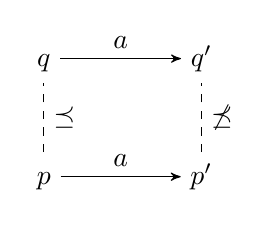
\begin{tikzpicture}[>=stealth']

    \node[] (q) {$\vphantom{A^1_1}q$};
    \node[below of=q,yshift=-5mm] (p) {$\vphantom{A^1_1}p$};
    \node[right of=q,xshift=10mm] (qprime) {$\vphantom{A^1_1}q'$};
    \node[below of=qprime,yshift=-5mm] (pprime) {$\vphantom{A^1_1}p'$};

    \draw[->] (p) edge node[above] {$a$} (pprime);
    \draw[->] (q) edge node[above] {$a$} (qprime);

    \draw[dashed] (p) edge node[right] {$\preceq$}(q);
    \draw[dashed] (pprime) edge node[right] {$\not\preceq$} (qprime);
    
  \end{tikzpicture}
\end{center}


%%%%%%%%%%%%%%%%%%%%%%%%%
\bibliographystyle{unsrt}
\bibliography{literature}
%%%%%%%%%%%%%%%%%%%%%%%%%

\end{document}
